\chapter{Estado del Arte: Arquitectura de Hyperledger Fabric y par\'ametros configurables}\label{chapter:state-of-the-art}

Hyperledger Fabric [\cite{HF}] es una de las plataformas blockchain m\'as populares administrada por Linux Foundation. Se basa en una plataforma privada de diferentes tipos de entidades, nodos pares, nodos ordenadores y clientes, pertenecientes a diferentes organizaciones. Cada una tiene una identidad en la red que es proporcionada por un Proveedor de Servicios de Membres\'ia $MSP$ [\cite{MSP}], generalmente asociado con una organizaci\'on. Todas las entidades de la red tienen visibilidad a las identidades de todas las organizaciones y pueden verificarlas. Difiere de las plataformas blockchain p\'ublicas que posibilitan la uni\'on de cualquier usuario a la red. Adem\'as, Fabric presenta una arquitectura de ejecuci\'on, orden y validaci\'on que supera los l\'imites de la arquitectura de orden y ejecuci\'on anterior [\cite{androulaki2018hyperledger}]. Esto mejora sustancialmente la escalabilidad de rendimiento en redes blockchain con un n\'umero elevado de nodos pares, lo que permite a Fabric ser competente en Global Trade Digitalization [\cite{digitizing-global}], SecureKey [\cite{securekey}] y Everledger [\cite{everledger}].Constituye la primera plataforma blockchain que admite contratos inteligentes creados en lenguajes de programaci\'on de uso general como Java, Golang y Node.js; siendo factible para la mayor\'ia de las empresas en el desarrollo de los contratos inteligentes, sin necesidad de capacidad adicional para aprender lenguajes espec\'ificos de dominio restringidos, conocidos por sus siglas en ingl\'es $DSL$. 

\section{Principales conceptos de Hyperledger Fabric}

\subsection{Chaincode}
El chaincode [\cite{chaincodes}] es un software que define uno o m\'as activos junto a las instrucciones de la transacci\'on para su modificaci\'on. Es el encargado de ofrecer la l\'ogica del negocio. Hace cumplir las reglas para leer o modificar los pares $llave-valor$ u otra informaci\'on de la base de datos de estado. Las funciones de un chaincode se ejecutan a partir de la base de datos del estado actual del libro mayor y se inician mediante una propuesta de transacci\'on dando como resultado un conjunto de escrituras $llave-valor$ que puede ser enviado a la red y aplicado al libro mayor en todos los nodos pares.

\subsection{Libro mayor}
El libro mayor o $ledger$ es un registro secuencial, a prueba de manipulaciones, de todas las transiciones de estado en Hyperledger Fabric. Las transiciones de estado son el resultado de los llamados del chaincode $(transacciones)$ presentadas por los miembros participantes. Cada transacci\'on da lugar a un conjunto de pares $llave-valor$ de activos que se registran en el libro mayor en forma de creaci\'on, actualizaci\'on o eliminaci\'on.

El libro mayor est\'a compuesto por una cadena de bloques para almacenar el registro inmutable y secuenciado en bloques, as\'i como una base de datos de estado para mantener el estado actual de Fabric. Existe un libro mayor por cada canal. Cada nodo par mantiene una copia del libro mayor para cada canal del que es miembro.

\subsection{Pol\'itica de aprobaci\'on}
Los chaincodes est\'an escritos en lenguajes de prop\'osito general que se ejecutan en nodos pares no confiables en la red. Por tanto, surgen m\'ultiples problemas, uno de car\'acter no determinista, ejecuci\'on, y el otro de confiar en los resultados de cualquier nodo par. La pol\'itica de aprobaci\'on aborda estas dos preocupaciones especificando como parte de una pol\'itica de aprobaci\'on, el conjunto de nodos pares que necesitan simular la transacci\'on y aprobar o firmar digitalmente los resultados de la ejecuci\'on.

\subsection{Sistema de chaincode}
Un sistema de chaincode tiene el mismo modelo de programaci\'on que los chaincodes de usuarios, pero est\'a integrado en el ejecutable del nodo par. Fabric implementa varios sistemas de chaincodes:
\begin{itemize}
\item Sistema de chaincode de ciclo de vida $(LSCC)$ permite instalar/crear instancias/actualizar chaincodes.

\item Sistema de chaincode de respaldo $(ESCC)$: permite aprobar una transacci\'on firmando digitalmente la respuesta.

\item Sistema chaincode de validaci\'on $(VSCC)$: posibilita evaluar la aprobaci\'on en la transacci\'on contra la pol\'itica de aprobaci\'on especificada para el chaincode. Si la pol\'itica de aprobaci\'on no se satisface, entonces la transacci\'on se toma como inv\'alida.

\item Control de Multiversi\'on de concurrencia [\cite{papadimitriou1984concurrency}] $MVCC$: garantiza que las versiones de las llaves le\'idas por una transacci\'on durante la fase de aprobaci\'on son igual que su estado actual en el libro mayor local en la fase de confirmaci\'on. Esto es similar a una verificaci\'on de conflicto de lectura y escritura realizada para el control de concurrencia, y se realiza secuencialmente en todas las transacciones v\'alidas en el bloque. Si las versiones del conjunto de lectura no coinciden, denota que anteriormente la transacci\'on modific\'o los datos le\'idos y fue desde su aprobaci\'on confirmada con \'exito, la transacci\'on es designada como inv\'alida. Para garantizar que no se produzcan lecturas fantasma la consulta se vuelve a ejecutar y se compara los $hashes$ de los resultados, que tambi\'en se almacena como parte del conjunto de lectura, capturado durante la aprobaci\'on.

\item Sistema de configuraci\'on chaincode $(CSCC)$: permite administrar las configuraciones de los canales.
\end{itemize}


\subsection{Canal}
Hyperledger Fabric introduce un concepto llamado $canal$ como una subred privada de comunicaci\'on entre dos o m\'as nodos pares para proporcionar un nivel de aislamiento. Las transacciones en un canal solo son vistos por sus nodos pares y participantes. El ledger y los chaincodes son definidos por canal. Adem\'as, el consenso es aplicable por canal, es decir, no hay un orden definido para la transacci\'on a trav\'es de los canales.

\subsection{Servicio de membres\'ia}
Un servicio de membres\'ia o $MSP$ abstrae todos los mecanismos y protocolos criptogr\'aficos detr\'as de la emisi\'on de certificados, la validaci\'on de certificados y la autenticaci\'on de usuarios. Un $MSP$ puede definir su propia noci\'on de identidad y las reglas por las cuales se rigen esas identidades (validaci\'on de identidad) y se autentican (generaci\'on y verificaci\'on de firmas).

Una red blockchain de Hyperledger Fabric puede estar gobernada por uno o m\'as $MSP$. Esto proporciona modularidad de las operaciones de membres\'ia e interoperabilidad entre diferentes est\'andares y arquitecturas.


\subsection{Nodo Par}
Un nodo par ejecuta el chaincode, que implementa un contrato inteligente del usuario y mantiene el ledger en un sistema de archivos. El chaincode tiene acceso permitido al estado compartido definido por la $API$. Entre los nodos pares se distinguen los que mantienen la l\'ogica del chaincode y lo ejecuta para aprobar una transacci\'on. Sin tener en consideraci\'on esta diferenciaci\'on, todos mantienen el libro mayor y el \'ultimo estado $StateDB$ en un registro de $llave-valor$ tal que se puede consultar o modificar el estado.

\subsection{Nodo Ordenador}
Los nodo ordenador participa en el protocolo de consenso y conforma el bloque de transacciones que se entrega a los nodos pares mediante un protocolo de comunicaci\'on $gossip$\footnote{El protocolo $Gossip$ es un protocolo que permite dise\~nar sistemas de comunicaciones distribuidos ($P2P$) altamente eficientes, seguros y de baja latencia.}. Juntos constituyen el servicio de ordenaci\'on, $OSN$ por sus siglas en ingl\'es, que posee un car\'acter modular y admite un mecanismo de consenso $conectable$. Se construye un bloque para ser entregado a los nodos pares, cuando se tenga un n\'umero m\'aximo de nuevas transacciones desde el \'ultimo bloque conformado, o se llegue al tiempo de espera configurado desde la \'ultima transacci\'on producida.

\subsection{Cliente}
Los clientes son responsables de llevar a cabo una propuesta de transacci\'on a uno o m\'as nodos pares simult\'aneamente para recopilar respuestas a propuestas y satisfacer la pol\'itica de aprobaci\'on. Posteriormente transmiten la transacci\'on al servicio de ordenaci\'on para ser incluida en un bloque y entregado a todos los pares para su validaci\'on y confirmaci\'on.

\section{Flujo de transacciones en Hyperledger Fabric}
A diferencia de otras redes Blockchain que emplean un modelo de $ordenaci\'on-ejecución$ [\cite{vukolic2017rethinking}] de transacciones, Fabric emplea un modelo de simulaci\'on, validaci\'on y confirmaci\'on de transacciones.\\ 

La figura \ref{flujo} muestra el flujo de la transacci\'on que consta de 3 fases:
\begin{itemize}
\item[1] Fase de aprobaci\'on: simular la transacci\'on en nodos pares selectivos y recopilar los cambios de estado.
\item[2] Fase de ordenaci\'on: ordenar las transacciones a trav\'es de un protocolo de consenso.
\item[3] Fase de validaci\'on: validaci\'on seguida de confirmaci\'on en el libro mayor.
\end{itemize}
\vspace{1 cm}
\begin{figure}
\centering
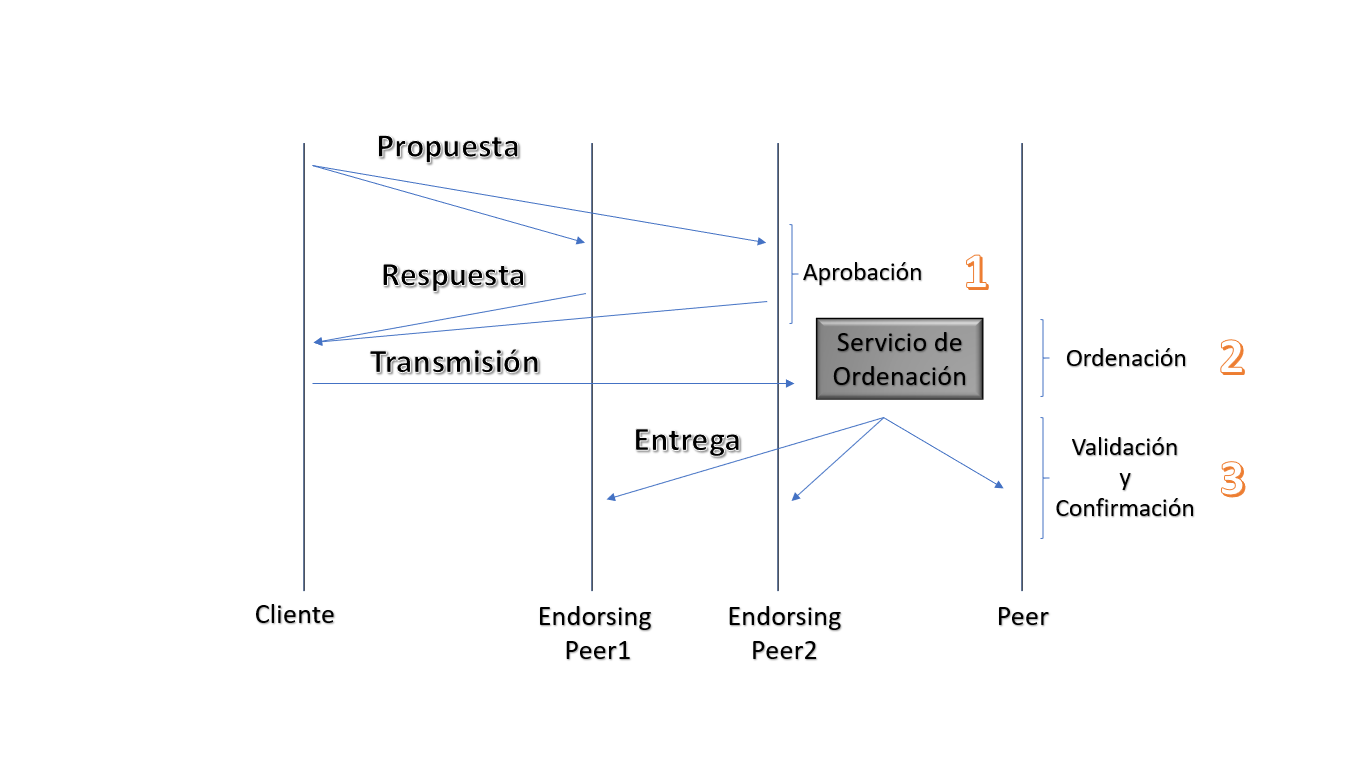
\includegraphics[width=0.6\linewidth]{Graphics/figura1.png}
\caption{Flujo de transacciones.}
\label{flujo}
\end{figure}
\vspace{1 cm}
Antes de que las transacciones sean enviadas, la red debe comenzar con las organizaciones participantes, sus $MSP$ e identidades de los nodos pares. Primero, se crea un canal en la red con los respectivos $MSP$ de las organizaciones. En segundo lugar, los nodos pares de cada organizaci\'on se unen al canal y se inicializa el libro mayor. Finalmente, los chaincodes requeridos se instalan en el canal.


\subsection{Fase de aprobaci\'on}
Una aplicaci\'on cliente que utiliza Fabric $SDK$ [\cite{Go-SDK}], [\cite{Node-SDK}], [\cite{Java-SDK}], construye una propuesta de transacci\'on para invocar un chaincode que a su vez realizar\'a operaciones en el estado del libro mayor. La propuesta est\'a firmada con las credenciales del cliente y el cliente lo env\'ia a uno o m\'as nodos pares simult\'aneamente. La pol\'itica de aprobaci\'on del chaincode dicta los nodos pares de la organizaci\'on que el cliente necesita para enviar la propuesta a la simulaci\'on. 
Primero, cada nodo par que aprueba, verifica que el remitente es autorizado para invocar transacciones en el canal. En segundo lugar, el nodo ejecuta el chaincode, que puede acceder al actual estado del libro mayor en el nodo par. Los resultados de la transacci\'on incluyen el valor de respuesta, conjunto de lectura y conjunto de escritura. En tercer lugar, el par que aprueba llama a un sistema chaincode llamado $ESCC$ que firma esta respuesta de transacci\'on con la identidad del nodo par y responde al cliente. Finalmente, el cliente inspecciona la respuesta de la propuesta a verificar que lleva la firma del nodo par. El cliente recoge las respuestas de diferentes nodos pares y verifica que sea la misma. Dado que cada nodo par pod\'ia haber ejecutado la transacci\'on en diferentes momentos en la Blockchain, es posible que la respuesta de la propuesta difiera. En tales casos, el cliente tiene que volver a enviar la propuesta a otros pares, para obtener suficientes respuestas coincidentes.

\subsection{Fase de ordenaci\'on}
El cliente transmite un mensaje de transacci\'on bien formado al servicio de ordenaci\'on. La transacci\'on tendr\'a los conjuntos de lectura y escritura, las firmas de los nodos pares que aprueban y la identificaci\'on del canal. El servicio de ordenaci\'on no necesita inspeccionar el contenido de la transacci\'on para realizar su operaci\'on. Recibe transacciones de diferentes clientes por varios canales y los pone en cola por canal. Crea bloques de transacciones por canal, firma el bloque con su identidad y los entrega a los nodos pares usando el protocolo de mensajer\'ia $gossip$.

\subsection{Fase de validaci\'on}
Todos los nodos pares en un canal reciben bloques de la red. Cada nodo par primero verifica la firma del nodo ordenador en el bloque. Cada bloque v\'alido se decodifica y todas las transacciones en un bloque pasan primero por una validaci\'on de $VSCC$ antes de realizar la validaci\'on de $MVCC$.

\subsection{Fase de actualizaci\'on en el libro mayor}
Como \'ultimo paso del procesamiento de transacciones, el libro mayor se actualiza agregando el bloque al libro mayor local $StateDB$, que contiene el estado actual de todas las llaves. Se actualiza con los conjuntos de escritura de transacciones v\'alidas. Estas actualizaciones de $StateDB$ se realizan para un bloque de transacciones y aplican las actualizaciones para llevar $StateDB$ al estado despu\'es de que se hayan procesado todas las transacciones en el bloque.

\section{Par\'ametros configurables}
Nuestro objetivo es estudiar el rendimiento de Fabric en diversas condiciones para comprender c\'omo las elecciones de las diferentes facetas del sistema afectan el rendimiento. Sin embargo, el espacio de par\'ametros es amplio y limitamos nuestras opciones para cubrir de manera integral algunos componentes y observar ampliamente otros aspectos del sistema para que podamos identificar la interacci\'on de las opciones de nivel de componente.

\subsection{Tama\~no de bloque}
Las transacciones se procesan por lotes en el nodo ordenador y entrega como un bloque a los nodos pares usando un protocolo $gossip$. Cada nodo par procesa un bloque a la vez. La variaci\'on del tama\~no de bloque tambi\'en trae consigo la compensaci\'on de rendimiento frente a latencia y, para obtener una mejor concepci\'on, lo estudiamos en conjunto con la tasa de llegada de transacciones.

\subsection{Pol\'itica de aprobaci\'on}
Una pol\'itica de aprobaci\'on dicta cu\'antas ejecuciones de una transacci\'on y firma deben ocurrir antes de que se pueda enviar una solicitud de transacci\'on al servicio de ordenaci\'on para que la transacci\'on pueda pasar la fase de validaci\'on $VSCC$ en los pares. La validaci\'on $VSCC$ de los aprobados de una transacci\'on requiere la evaluaci\'on de la expresi\'on de la pol\'itica de aprobaci\'on frente a los aprobados recopilados y la verificaci\'on de la satisfacibilidad [\cite{gottlieb2002evolutionary}], que es $NP-Completo$. Adicionalmente, incluye verificar la identidad y su firma. La complejidad de la pol\'itica de aprobaci\'on afectar\'a los recursos y el tiempo necesario para recopilar y evaluar transacciones.

\subsection{Canal}
Los canales a\'islan las transacciones. Las transacciones enviadas a diferentes canales se ordenan, entregan y procesan de forma independiente, aunque en el mismo nodo par. Los canales aportan un paralelismo inherente a varios aspectos de procesamiento de transacciones en Hyperledger Fabric. Mientras que el n\'umero de canales a emplear, y en qu\'e canales realizar transacciones est\'a determinado por la aplicaci\'on y la combinatoria de los participantes, tiene importantes implicaciones en el rendimiento y la escalabilidad de la plataforma.

\subsection{Recursos}
Los nodos pares ejecutan la firma y verificaci\'on como parte de un sistema chaincode con empleo intensivo de la $CPU$.

\subsection{Base de datos del libro mayor}
Fabric admite dos alternativas para almacenar $llave-valor$, $CouchDB$ [\cite{CouchDB}] y $GoLevelDB$ [\cite{GoLevelDB}] para mantener el estado actual. Ambos almacenan $llave-valor$, mientras que $GoLevelDB$ es una base de datos incrustada, $CouchDB$ usa un modelo $cliente-servidor$ (al que se accede mediante la $API$ $REST$ a trav\'es de un $HTTPS$) y es compatible con documentos $JSON$.

\section{Hyperledger Fabric v2.x}
La primera versi\'on de notoria importancia de Hyperledger Fabric luego de su lanzamiento con la versi\'on 1.0 fue Fabric v2.0. Ofrece nuevas caracter\'isticas y cambios representativos para usuarios y operadores. Incluye la compatibilidad con nuevos patrones de aplicaciones y privacidad, gobernanza mejorada en torno a contratos inteligentes y nuevas opciones para nodos operativos.\\

Fabric v2.0 presenta un gobierno descentralizado para contratos inteligentes, con un nuevo proceso para instalar un chaincode en sus nodos pares e instanciarlos en un canal. El nuevo ciclo de vida del chaincode de Fabric permite que varias organizaciones lleguen a un acuerdo sobre los par\'ametros del chaincode, como la pol\'itica de aprobaci\'on del contrato, antes de que pueda usarse para interactuar con el ledger. El nuevo modelo ofrece varias mejoras con respecto al ciclo de vida anterior [\cite{hyperledger2018hyperledger}]:

{\begin{itemize}
\item {\bf M\'ultiples organizaciones deben aceptar los par\'ametros de un chaincode}. En las versiones de lanzamiento 1.x, una organizaci\'on ten\'ia la capacidad de establecer par\'ametros de un chaincode, como la pol\'itica de aprobaci\'on, para todos los miembros del canal, que solo ten\'ian el poder de negarse a instalar el chaincode, por lo tanto, no participar en transacciones que lo invoquen. El nuevo ciclo de vida del chaincode de Fabric es m\'as flexible, admite tanto el modelo de ciclo de vida anterior, como modelos descentralizados que requieren suficiente n\'umero de organizaciones para acordar una pol\'itica de aprobaci\'on y otros detalles antes de que el chaincode se convierta en activo en un canal.

\item {\bf Proceso de actualizaci\'on de chaincode m\'as deliberado}. Anteriormente la transacci\'on de actualizaci\'on pod\'ia ser emitida por una sola organizaci\'on, creando un riesgo para un miembro del canal que a\'un no hab\'ia instalado el nuevo chaincode. El nuevo modelo permite que el chaincode se actualice solo despu\'es de que un n\'umero suficiente de organizaciones han aprobado la actualizaci\'on.

\item {\bf Actualizaciones m\'as sencillas de pol\'iticas de respaldo y recopilaci\'on de datos privados}. Se permite cambiar una pol\'itica de respaldo o una configuraci\'on de recopilaci\'on de datos privados sin tener que volver a empaquetar o instalar el chaincode. Los usuarios tambi\'en pueden aprovechar una nueva pol\'itica de aprobaci\'on predeterminada que requiere la aprobaci\'on de una mayor\'ia de organizaciones en el canal. Esta pol\'itica se actualiza autom\'aticamente cuando se agregan o eliminan organizaciones del canal.

\item {\bf Paquetes de chaincodes inspeccionables}. El chaincode se empaqueta en archivos {\bf .tar} f\'aciles de leer, que hace m\'as factible su inspecci\'on  y coordinaci\'on de la instalaci\'on en m\'ultiples organizaciones.

\item {\bf Iniciar m\'ultiples chaincodes en un canal usando un paquete}. El ciclo de vida anterior defin\'ia cada chaincode en el canal usando un nombre y una versi\'on que se especific\'o en su instalaci\'on. Ahora existe la posibilidad de usar un solo paquete de chaincodes y desplegarlo varias veces con diferentes nombres en el mismo canal o en diferentes canales.
\end{itemize}

Los mismos m\'etodos descentralizados para llegar a un acuerdo que sustentan la nueva gesti\'on del ciclo de vida del chaincode pueden usarse tambi\'en en su propia aplicaci\'on para garantizar que las organizaciones den su consentimiento a las transacciones de datos antes de que se realicen escrituras en el libro mayor.\\

\begin{itemize}
\item {\bf Comprobaciones automatizadas}. Las organizaciones pueden agregar comprobaciones autom\'aticas a las funciones del chaincode para validar informaci\'on adicional antes de aprobar una propuesta de transacci\'on.

\item {\bf Acuerdo descentralizado}. Las decisiones humanas se pueden modelar en un proceso de chaincode que abarca m\'ultiples transacciones. El chaincode puede requerir que los actores de varias organizaciones indiquen sus t\'erminos y condiciones de acuerdo en una transacci\'on en el libro mayor. Luego, una propuesta final de chaincode puede verificar que las condiciones de todas las transacciones individuales se cumplen y establecer la transacci\'on comercial con car\'acter definitivo en todos los miembros del canal.
\end{itemize}

Fabric v2.0 tambi\'en permite nuevos patrones para trabajar y compartir datos privados, sin el requisito de crear recopilaciones de datos privados para todas las combinaciones de miembros del canal que deseen realizar transacciones. Espec\'ificamente, en lugar de compartir datos privados dentro de una colecci\'on de varios miembros. Es posible compartir datos privados entre colecciones, donde cada colecci\'on puede incluir una sola organizaci\'on, o tal vez una sola organizaci\'on junto con un regulador o auditor.\\

\begin{itemize}
\item {\bf Compartir y verificar datos privados}. Cuando los datos privados se comparten con un miembro del canal que no es miembro de una colecci\'on, o compartida con otra colecci\'on de datos privados que contiene uno o m\'as miembros del canal (escribiendo una llave para esa colecci\'on), las partes receptoras pueden utilizar la $API$ del chaincode $GetPrivateDataHash()$ para verificar que los datos privados coincidan con los $hash$ en la cadena que se crearon a partir de datos privados en transacciones anteriores.

\item {\bf Pol\'iticas de aprobaci\'on a nivel de colecci\'on}. Las colecciones de datos privados ahora se pueden definir opcionalmente con una pol\'itica de aprobaci\'on que anula la pol\'itica de aprobaci\'on a nivel de chaincode para las llaves dentro de la colecci\'on. Se puede usar para restringir qu\'e organizaciones pueden escribir datos en una colecci\'on. Se puede concebir un chaincode que requiere el respaldo de la mayor\'ia de las organizaciones, pero para cualquier transacci\'on determinada, puede necesitar dos organizaciones transaccionales para respaldar individualmente su acuerdo en sus propias colecciones de datos privados.

\item {\bf Recopilaciones impl\'icitas por organizaci\'on}. Si se desea utilizar patrones de datos privados por organizaci\'on, no se necesita definir las colecciones al implementar chaincode. Las colecciones se pueden usar sin ninguna definici\'on inicial.
\end{itemize}

La funci\'on de lanzador de chaincode externo permite a los operadores crear y lanzar chaincode con la tecnolog\'ia de su elecci\'on. No se requiere el uso de constructores y lanzadores externos ya que el comportamiento predeterminado construye y ejecuta el chaincode de la misma manera que las versiones anteriores con la $API$ de Docker.

\begin{itemize}

\item {\bf Elimina la dependencia del demonio de Docker}. Las versiones anteriores de Fabric requer\'ian que los nodos pares tuvieran acceso a un $Docker daemon$  para construir y lanzar chaincode, algo que puede no ser deseable en entornos de producci\'on.

\item {\bf Alternativas a los contenedores}. Ya no es necesario ejecutar chaincode en contenedores Docker, y puede ejecutarse en el entorno elegido por el operador (incluidos los contenedores).


\item {\bf Chaincode como un servicio externo}. Tradicionalmente, los chaincodes son lanzados por el nodo par y luego se conectan de nuevo a \'el. Ahora es posible ejecutar chaincode como un servicio externo, por ejemplo, en un $pod$ de Kubernetes, que un nodo par puede conectarse y utilizar para la ejecuci\'on de chaincode.
\end{itemize}

Cuando se utiliza una base de datos de estado externa $CouchDB$, los retrasos de lectura durante las fases de aprobaci\'on y validaci\'on han representado un cuello de botella en el rendimiento. Con Fabric v2.0, una nueva cach\'e reemplaza muchas de estas costosas b\'usquedas con lecturas r\'apidas de cach\'e local. El tama\~no de cach\'e se configura mediante la propiedad $cacheSize$ en $core.yaml$.\\